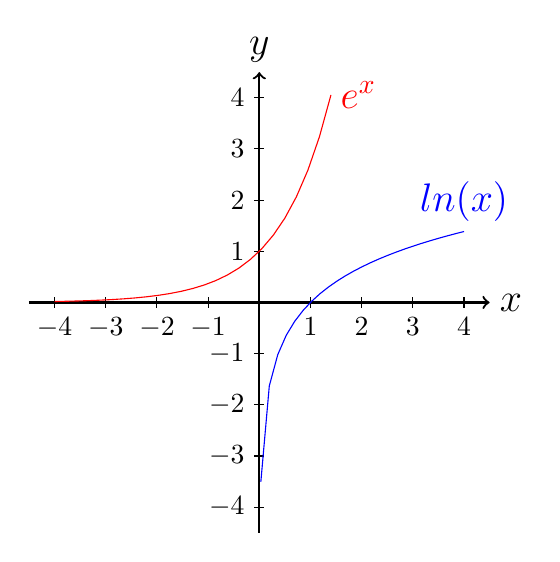
\begin{tikzpicture}[xscale=0.65, yscale=0.65]
	%axis
	\draw[thick, ->] (-4.5, 0) -- (4.5,0) node[right] {\Large $x$};
	\draw[thick, ->] (0, -4.5) -- (0,4.5) node[above] {\Large $y$};
	%
	%grid x
	\draw (-4, -0.1) node[below]{$-4$} -- (-4, 0.1);
	\draw (-3, -0.1) node[below]{$-3$} -- (-3, 0.1);
	\draw (-2, -0.1) node[below]{$-2$} -- (-2, 0.1);
	\draw (-1, -0.1) node[below]{$-1$} -- (-1, 0.1);
	\draw (1, -0.1) node[below]{$1$} -- (1, 0.1);
	\draw (2, -0.1) node[below]{$2$} -- (2, 0.1);
	\draw (3, -0.1) node[below]{$3$} -- (3, 0.1);
	\draw (4, -0.1) node[below]{$4$} -- (4, 0.1);
	%grid y
	\draw (-0.1, 4) node[left]{$4$} -- (0.1, 4);
	\draw (-0.1, 3) node[left]{$3$} -- (0.1, 3);
	\draw (-0.1, 2) node[left]{$2$} -- (0.1, 2);
	\draw (-0.1, 1) node[left]{$1$} -- (0.1, 1);
	\draw (-0.1, -1) node[left]{$-1$} -- (0.1, -1);
	\draw (-0.1, -2) node[left]{$-2$} -- (0.1, -2);
	\draw (-0.1, -3) node[left]{$-3$} -- (0.1, -3);
	\draw (-0.1, -4) node[left]{$-4$} -- (0.1, -4);
	%
	%plots
	\draw[red, domain=-4:1.4] plot (\x, {e^\x}) node[right, red] {\Large $e^x$};
	\draw[blue, domain=0.03:4] plot (\x, {ln(\x)})node[above, blue] {\Large $ln(x)$};
\end{tikzpicture}